\chapter{Introduction}
Machine learning design methodologies to extract patterns from data, ideally without much domain-specific expertise and it is made with a lot different parts like Big Data, computer science, statistics and other.
\begin{figure}[H]
    \centering
    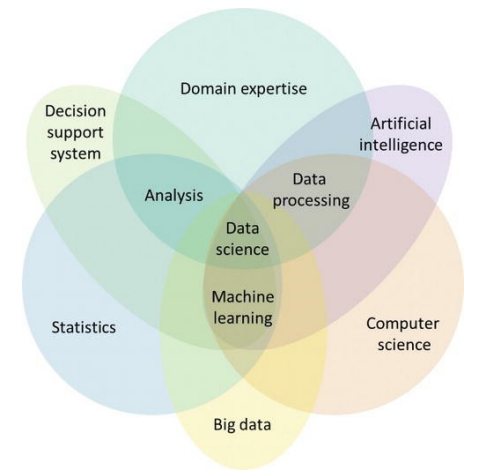
\includegraphics[scale=0.5]{images/Introduction/Intro1.png}
    \caption{Different part of machine learning and more}
    \label{fig:enter-label}
\end{figure}

Big Data are data whose scale, diversity and complexity require new architectures, techniques, algorithms and analytics to manage it and extract value and hidden knowledge from it.
That are made with 5 V:
\begin{itemize}
    \item \textbf{Volume}, as the name can say Big data work with incredible volume of data that exponentially increase over time
    \item \textbf{Velocity}, there is some fast data with fast generation rate so we have to analyse them very fast
    \item \textbf{Variety}, the data can have various formats, types and structures like audio,video, text, or packet
    \item \textbf{Veracity}, the data quality compromised by misrepresented data, outlier, software bug and so on.
    \item \textbf{Value}, all the data has to be transform in something useful in decision making and to gain a business advantage
\end{itemize}

Instead Data Science is about extracting meaning from large quantities of data, taking the raw data then cleaning them and finally apply Machine learning to create model.
The data can be generated or acquired and both have to be stored in some infrastructure, file system or programming models. After that starts the preprocessing part divided in 2: data cleaning and integration. Both parts are needed to have better data solving inconsistencies and unifying information from different sources or managing conflicts and redundancy

Machine learning is all about fit models to data to make prediction or forecasts and there is two different ways, one is supervised learning or Classification/Regression, and the other one is Unsupervised learning or Clustering

\begin{figure}[H]
    \centering
    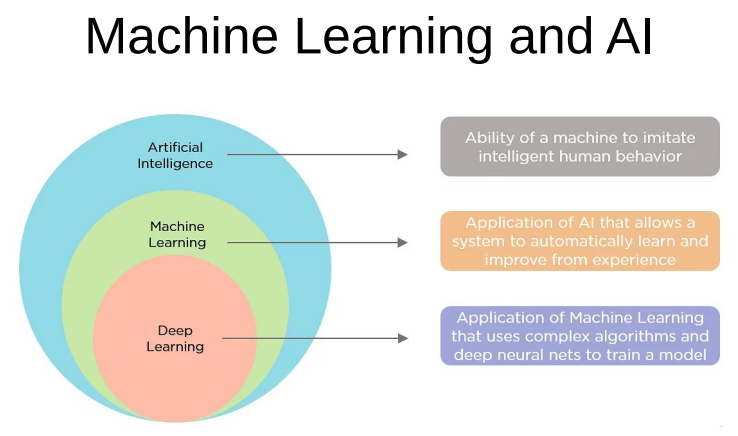
\includegraphics[scale=0.5]{images/Introduction/Intro2.png}
    \caption{Machine learning}
    \label{fig:enter-label}
\end{figure}